\def\fullversionflag{0}

\ifodd\fullversionflag
    \documentclass[letterpaper,11pt]{article}
\else
    \documentclass{llncs}
\fi

\usepackage{etoolbox}
\newtoggle{fullversion}
\ifodd\fullversionflag
    \toggletrue{fullversion}
\else
    \togglefalse{fullversion}
\fi

\usepackage[pdfstartview=FitH,colorlinks,urlcolor=black,linkcolor=black,citecolor=black,pdfpagelabels]{hyperref}
\usepackage[usenames,dvipsnames]{color}
%\usepackage{times}
\usepackage{microtype,pdfsync}
\usepackage{graphicx}
\iftoggle{fullversion}{
\usepackage{amsthm}}{}
\usepackage{amsmath,amsfonts,amssymb}
\usepackage{tabu} % detect if table is in math mode
\usepackage{url} \usepackage{graphicx}
\iftoggle{fullversion}{
\usepackage{fullpage}}{}
\usepackage{mathtools}
\usepackage{footnote}

\newcommand{\Theorem}[1]{\hyperref[#1]{Theorem~\ref*{#1}}}
\newcommand{\Lemma}[1]{\hyperref[#1]{Lemma~\ref*{#1}}}
\newcommand{\Corollary}[1]{\hyperref[#1]{Corollary~\ref*{#1}}}
\newcommand{\Definition}[1]{\hyperref[#1]{Definition~\ref*{#1}}}
\newcommand{\Conjecture}[1]{\hyperref[#1]{Conjecture~\ref*{#1}}}
\newcommand{\Section}[1]{\hyperref[#1]{Section~\ref*{#1}}}
\newcommand{\Appendix}[1]{\hyperref[#1]{Appendix~\ref*{#1}}}

%\usepackage{natbib}
%\setlength{\bibsep}{0.3em}

\usepackage{xspace}
\usepackage{multirow}
\usepackage{enumitem}

\usepackage[hang,flushmargin]{footmisc}

\usepackage{tikz}
\usetikzlibrary{calc,positioning,shapes,shadows,arrows,fit}

\newcommand{\ignore}[1]{}

\usepackage{caption}
\captionsetup[figure]{width=.86\textwidth}
\captionsetup[table]{width=.86\textwidth}
\setlength{\abovecaptionskip}{0pt}
\setlength{\belowcaptionskip}{3pt}

\newenvironment{vbx}{\vbox\bgroup}{\egroup}

\numberwithin{equation}{section}

%fields and groups
\newcommand{\F}{\mathbb{F}}
\newcommand{\Q}{\mathbb{Q}} 
\newcommand{\N}{\mathbb{N}}
\newcommand{\Z}{\mathbb{Z}}
\newcommand{\R}{\mathbb{R}} 
\newcommand{\C}{\mathbb{C}}
\newcommand{\Qbar}{\overline{\Q}} 
\newcommand{\G}{\mathbb{G}}
\newcommand{\Vs}{\mathbb{V}} 
\newcommand{\Fbar}{\overline{\mathbb{F}}}

%vectors, etc.
\newcommand{\av}{\mathbf{a}} \newcommand{\cv}{\mathbf{c}} 
\newcommand{\dv}{\mathbf{d}} \newcommand{\ev}{\mathbf{e}} 
\newcommand{\rv}{\mathbf{r}} \newcommand{\sv}{\mathbf{s}} 
\newcommand{\tv}{\mathbf{t}} \newcommand{\uv}{\mathbf{u}} 
\newcommand{\vv}{\mathbf{v}} \newcommand{\wv}{\mathbf{w}} 
\newcommand{\xv}{\mathbf{x}} \newcommand{\yv}{\mathbf{y}} 
\newcommand{\zv}{\mathbf{z}} \newcommand{\zerov}{\mathbf{0}}
\renewcommand{\AA}{\mathbf{A}} \newcommand{\BB}{\mathbf{B}} 
\newcommand{\CC}{\mathbf{C}} \newcommand{\FF}{\mathbf{F}} 
\newcommand{\MM}{\mathbf{M}} \newcommand{\RR}{\mathbf{R}} 
\renewcommand{\SS}{\mathbf{S}} \newcommand{\TT}{\mathbf{T}} 
\newcommand{\UU}{\mathbf{U}} \newcommand{\XX}{\mathcal{X}} 
\newcommand{\YY}{\mathcal{Y}} \newcommand{\KK}{\mathcal{K}} 
\newcommand{\A}{\mathcal{A}} \newcommand{\B}{\mathcal{B}} 
\newcommand{\dash}{\mbox{---}}
\renewcommand{\O}{\mathcal{O}}
\newcommand{\qq}{\mathfrak{q}}
\newcommand{\QQ}{\mathfrak{Q}}
\newcommand{\ZQ}{\Z_{q}}

\newcommand{\vtbl}[2]{\begin{array}{c}
\hspace*{-3pt} #1 \hspace*{-4pt} \vspace*{5pt} \\
\hspace*{-3pt} #2 \hspace*{-4pt}
\end{array}}

%\newcommand{\vk}{\mathbf{k}}
\newcommand{\vu}{\mathbf{u}}

\newcommand{\todo}[1]{{\color{red} {\bf TODO}:~{#1}}}
\newcommand{\btodo}[1]{{\color{blue} {\bf TODO}:~{#1}}}
\newcommand{\ltodo}[2]{{\color{blue} {\bf TODO (locked by {#1})}:~{#2}}}
\newcommand{\lbtodo}[2]{{\color{blue} {\bf TODO (locked by {#1}}:~{#2}}}

\newcommand{\mr}[1]{\ensuremath{\mathrm{{#1}}}}
\newcommand{\la}{\ensuremath{\leftarrow}}
\newcommand{\ra}{\ensuremath{\rightarrow}}
\newcommand{\ala}{\ensuremath{\ \la\ }}
\newcommand{\ara}{\ensuremath{\ \ra\ }}
\newcommand{\rf}{\ensuremath{\overset{\$}{\la}}}

\newcommand{\dist}[1]{\esm{\left\langle{#1}\right\rangle}}

\newcommand{\parh}[1]{{\bf {#1}}\ \ }
\renewcommand{\paragraph}[1]{\medskip\noindent {\bf {#1}}}


\newcommand{\calA}{\ensuremath{\mathcal{A}}}
\newcommand{\calB}{\ensuremath{\mathcal{B}}}
\newcommand{\calC}{\ensuremath{\mathcal{C}}}
\newcommand{\calD}{\ensuremath{\mathcal{D}}}
\newcommand{\calE}{\ensuremath{\mathcal{E}}}
\newcommand{\calF}{\ensuremath{\mathcal{F}}}
\newcommand{\calG}{\ensuremath{\mathcal{G}}}
\newcommand{\calH}{\ensuremath{\mathcal{H}}}
\newcommand{\calI}{\ensuremath{\mathcal{I}}}
\newcommand{\calJ}{\ensuremath{\mathcal{J}}}
\newcommand{\calK}{\ensuremath{\mathcal{K}}}
\newcommand{\calL}{\ensuremath{\mathcal{L}}}
\newcommand{\calM}{\ensuremath{\mathcal{M}}}
\newcommand{\calN}{\ensuremath{\mathcal{N}}}
\newcommand{\calO}{\ensuremath{\mathcal{O}}}
\newcommand{\calP}{\ensuremath{\mathcal{P}}}
\newcommand{\calQ}{\ensuremath{\mathcal{Q}}}
\newcommand{\calR}{\ensuremath{\mathcal{R}}}
\newcommand{\calS}{\ensuremath{\mathcal{S}}}
\newcommand{\calT}{\ensuremath{\mathcal{T}}}
\newcommand{\calU}{\ensuremath{\mathcal{U}}}
\newcommand{\calV}{\ensuremath{\mathcal{V}}}
\newcommand{\calW}{\ensuremath{\mathcal{W}}}
\newcommand{\calX}{\ensuremath{\mathcal{X}}}
\newcommand{\calY}{\ensuremath{\mathcal{Y}}}
\newcommand{\calZ}{\ensuremath{\mathcal{Z}}}

% -- bold math symbols, for some reason --
\newcommand{\boldalpha}{\ensuremath{\boldsymbol{\alpha}}}
\newcommand{\boldchi}{\ensuremath{\boldsymbol{\chi}}}
\newcommand{\boldtau}{\ensuremath{{\boldsymbol{\tau}}}}
\newcommand{\boldstar}{\ensuremath{\mathbf{*}}}
\newcommand{\bolda}{\ensuremath{\mathbf{a}}}
\newcommand{\boldb}{\ensuremath{\mathbf{b}}}
\newcommand{\boldc}{\ensuremath{\mathbf{c}}}
\newcommand{\boldd}{\ensuremath{\mathbf{d}}}
\newcommand{\bolde}{\ensuremath{\mathbf{e}}}
\newcommand{\boldf}{\ensuremath{\mathbf{f}}}
\newcommand{\boldg}{\ensuremath{\mathbf{g}}}
\newcommand{\boldh}{\ensuremath{\mathbf{h}}}
\newcommand{\boldi}{\ensuremath{\mathbf{i}}}
\newcommand{\boldj}{\ensuremath{\mathbf{j}}}
\newcommand{\boldk}{\ensuremath{\mathbf{k}}}
\newcommand{\boldl}{\ensuremath{\mathbf{l}}}
\newcommand{\boldm}{\ensuremath{\mathbf{m}}}
\newcommand{\boldn}{\ensuremath{\mathbf{n}}}
\newcommand{\boldo}{\ensuremath{\mathbf{o}}}
\newcommand{\boldp}{\ensuremath{\mathbf{p}}}
\newcommand{\boldq}{\ensuremath{\mathbf{q}}}
\newcommand{\boldr}{\ensuremath{\mathbf{r}}}
\newcommand{\bolds}{\ensuremath{\mathbf{s}}}
\newcommand{\boldt}{\ensuremath{\mathbf{t}}}
\newcommand{\boldu}{\ensuremath{\mathbf{u}}}
\newcommand{\boldv}{\ensuremath{\mathbf{v}}}
\newcommand{\boldw}{\ensuremath{\mathbf{w}}}
\newcommand{\boldx}{{\ensuremath{\mathbf{x}}}}
\newcommand{\boldy}{\ensuremath{\mathbf{y}}}
\newcommand{\boldz}{\ensuremath{\mathbf{z}}}
\newcommand{\boldzero}{\ensuremath{\boldsymbol{0}}}
\newcommand{\boldone}{\ensuremath{\boldsymbol{1}}}

% -- bold italic math symbols, for some reason --
\newcommand{\boldia}{\ensuremath{\boldsymbol{a}}}
\newcommand{\boldib}{\ensuremath{\boldsymbol{b}}}
\newcommand{\boldic}{\ensuremath{\boldsymbol{c}}}
\newcommand{\boldid}{\ensuremath{\boldsymbol{d}}}
\newcommand{\boldie}{\ensuremath{\boldsymbol{e}}}
\newcommand{\boldif}{\ensuremath{\boldsymbol{f}}}
\newcommand{\boldig}{\ensuremath{\boldsymbol{g}}}
\newcommand{\boldih}{\ensuremath{\boldsymbol{h}}}
\newcommand{\boldii}{\ensuremath{\boldsymbol{i}}}
\newcommand{\boldij}{\ensuremath{\boldsymbol{j}}}
\newcommand{\boldik}{\ensuremath{\boldsymbol{k}}}
\newcommand{\boldil}{\ensuremath{\boldsymbol{l}}}
\newcommand{\boldim}{\ensuremath{\boldsymbol{m}}}
\newcommand{\boldin}{\ensuremath{\boldsymbol{n}}}
\newcommand{\boldio}{\ensuremath{\boldsymbol{o}}}
\newcommand{\boldip}{\ensuremath{\boldsymbol{p}}}
\newcommand{\boldiq}{\ensuremath{\boldsymbol{q}}}
\newcommand{\boldir}{\ensuremath{\boldsymbol{r}}}
\newcommand{\boldis}{\ensuremath{\boldsymbol{s}}}
\newcommand{\boldit}{\ensuremath{\boldsymbol{t}}}
\newcommand{\boldiu}{\ensuremath{\boldsymbol{u}}}
\newcommand{\boldiv}{\ensuremath{\boldsymbol{v}}}
\newcommand{\boldiw}{\ensuremath{\boldsymbol{w}}}
\newcommand{\boldix}{\ensuremath{\boldsymbol{x}}}
\newcommand{\boldiy}{\ensuremath{\boldsymbol{y}}}
\newcommand{\boldiz}{\ensuremath{\boldsymbol{z}}}

\newcommand{\transpose}[1]{\ensuremath{{#1}^{\intercal}}}

\newcommand{\boldA}{\ensuremath{\mathbf{A}}}
\newcommand{\boldB}{\ensuremath{\mathbf{B}}}
\newcommand{\boldC}{\ensuremath{\mathbf{C}}}
\newcommand{\boldD}{\ensuremath{\mathbf{D}}}
\newcommand{\boldE}{\ensuremath{\mathbf{E}}}
\newcommand{\boldF}{\ensuremath{\mathbf{F}}}
\newcommand{\boldG}{\ensuremath{\mathbf{G}}}
\newcommand{\boldH}{\ensuremath{\mathbf{H}}}
\newcommand{\boldI}{\ensuremath{\mathbf{I}}}
\newcommand{\boldJ}{\ensuremath{\mathbf{J}}}
\newcommand{\boldK}{\ensuremath{\mathbf{K}}}
\newcommand{\boldL}{\ensuremath{\mathbf{L}}}
\newcommand{\boldM}{\ensuremath{\mathbf{M}}}
\newcommand{\boldN}{\ensuremath{\mathbf{N}}}
\newcommand{\boldO}{\ensuremath{\mathbf{O}}}
\newcommand{\boldP}{\ensuremath{\mathbf{P}}}
\newcommand{\boldQ}{\ensuremath{\mathbf{Q}}}
\newcommand{\boldR}{\ensuremath{\mathbf{R}}}
\newcommand{\boldS}{\ensuremath{\mathbf{S}}}
\newcommand{\boldT}{\ensuremath{\mathbf{T}}}
\newcommand{\boldU}{\ensuremath{\mathbf{U}}}
\newcommand{\boldV}{\ensuremath{\mathbf{V}}}
\newcommand{\boldW}{\ensuremath{\mathbf{W}}}
\newcommand{\boldX}{\ensuremath{\mathbf{X}}}
\newcommand{\boldY}{\ensuremath{\mathbf{Y}}}
\newcommand{\boldZ}{\ensuremath{\mathbf{Z}}}

\newcommand{\bbA}{\ensuremath{\mathbb{A}}}
\newcommand{\bbB}{\ensuremath{\mathbb{B}}}
\newcommand{\bbC}{\ensuremath{\mathbb{C}}}
\newcommand{\bbD}{\ensuremath{\mathbb{D}}}
\newcommand{\bbE}{\ensuremath{\mathbb{E}}}
\newcommand{\bbF}{\ensuremath{\mathbb{F}}}
\newcommand{\bbG}{\ensuremath{\mathbb{G}}}
\newcommand{\bbH}{\ensuremath{\mathbb{H}}}
\newcommand{\bbI}{\ensuremath{\mathbb{I}}}
\newcommand{\bbJ}{\ensuremath{\mathbb{J}}}
\newcommand{\bbK}{\ensuremath{\mathbb{K}}}
\newcommand{\bbL}{\ensuremath{\mathbb{L}}}
\newcommand{\bbM}{\ensuremath{\mathbb{M}}}
\newcommand{\bbN}{\ensuremath{\mathbb{N}}}
\newcommand{\bbO}{\ensuremath{\mathbb{O}}}
\newcommand{\bbP}{\ensuremath{\mathbb{P}}}
\newcommand{\bbQ}{\ensuremath{\mathbb{Q}}}
\newcommand{\bbR}{\ensuremath{\mathbb{R}}}
\newcommand{\bbS}{\ensuremath{\mathbb{S}}}
\newcommand{\bbT}{\ensuremath{\mathbb{T}}}
\newcommand{\bbU}{\ensuremath{\mathbb{U}}}
\newcommand{\bbV}{\ensuremath{\mathbb{V}}}
\newcommand{\bbW}{\ensuremath{\mathbb{W}}}
\newcommand{\bbX}{\ensuremath{\mathbb{X}}}
\newcommand{\bbY}{\ensuremath{\mathbb{Y}}}
\newcommand{\bbZ}{\ensuremath{\mathbb{Z}}}

\newcommand{\deq}{\mathrel{\mathop:}=}
%\newcommand{\deq}{\ensuremath{\stackrel{\sf def}{=}}} % defined as equal to
\newcommand{\zo}{\ensuremath{\{0,1\}}} % bits


% THEOREMS %%%%%%%%%%%%%%%%%%%%%%%%%%%%%%%%%%%%%%%%%%%%%%%%%%%%%%%%%%%%%%%%%%%
%
% Theorem definitions

\iftoggle{fullversion}{
\theoremstyle{plain} \newtheorem{theorem}{Theorem}[section] 
\newtheorem{lemma}[theorem]{Lemma}
\newtheorem{claim}[theorem]{Claim}
\newtheorem{remark}[theorem]{Remark}
\newtheorem{proposition}[theorem]{Proposition} 
\newtheorem{corollary}[theorem]{Corollary}

\theoremstyle{definition} \newtheorem{defn}[theorem]{Definition} 
\newtheorem{definition}[theorem]{Definition} \newtheorem{rem}[theorem]{Remark} 
%\newtheorem{alg}[theorem]{Algorithm} 
\newtheorem{fact}[theorem]{Fact}
%\newtheorem{construction}[theorem]{Construction} 
}{}


%% custom macros


\newcommand{\esm}[1]{\ensuremath{#1}}
\newcommand{\ms}[1]{\esm{\mathsf{#1}}}

\newcommand{\Am}{\mathbf{A}}
\newcommand{\Um}{\mathbf{U}}

\newcommand{\LWE}{\ms{LWE}}

\newcommand{\perplattice}{\Lambda_q^{\bot}}
\newcommand{\cosetlattice}[1]{\Lambda_q^{#1}}

\newcommand{\set}[1]{\{ #1 \}}
\newcommand{\getsdollar}{\overset{\$}{\gets}}
\newcommand{\poly}{\ms{poly}}
\newcommand{\negl}{\ms{negl}}


\newcommand{\PiFHE}{\Pi_{\ms{FHE}}}
\newcommand{\FHEKeyGen}{\ms{FHE.KeyGen}}
\newcommand{\FHEEnc}{\ms{FHE.Enc}}
\newcommand{\FHEEval}{\ms{FHE.Eval}}
\newcommand{\FHEDec}{\ms{FHE.Dec}}

\newcommand{\sk}{\ms{sk}}
\newcommand{\ct}{\ms{ct}}
\newcommand{\msk}{\ms{msk}}
\newcommand{\pp}{\ms{pp}}
\newcommand{\state}{\ms{state}}

\newcommand{\PiPRF}{\Pi_\ms{pPRF}}
\newcommand{\PRFSetup}{\ms{pPRF.Setup}}
\newcommand{\PRFPuncture}{\ms{pPRF.Puncture}}
\newcommand{\PRFPunctureEval}{\ms{pPRF.PunctureEval}}
\newcommand{\PRFEval}{\ms{pPRF.Eval}}

\newcommand{\Bm}{\mathbf{B}}
\newcommand{\Cm}{\mathbf{C}}
\newcommand{\Dm}{\mathbf{D}}
\newcommand{\Identity}{\mathbf{I}}

\newcommand{\Rm}{\mathbf{R}}
\newcommand{\Gm}{\mathbf{G}}
\newcommand{\mv}{\mathbf{m}}
\newcommand{\bv}{\mathbf{b}}
\newcommand{\kv}{\mathbf{k}}
\newcommand{\Mm}{\mathbf{M}}
\newcommand{\kS}{k_{\scriptscriptstyle S}}

\newcommand{\gv}{\mathbf{g}}

\newcommand{\noise}{\ms{noise}}

\newcommand{\FHEpp}{\ms{fhe.pp}}
\newcommand{\FHEsk}{\ms{fhe.sk}}
\newcommand{\FHEct}{\ms{fhe.ct}}

\newcommand{\iprod}[2]{\left\langle #1, #2 \right\rangle}


\newcommand{\evalcomp}{\ms{Eval}_{\ms{comp},j}}
\newcommand{\comp}{\ms{comp}}
\newcommand{\roundp}[1]{\lfloor #1 \rceil_p}

\newcommand{\evalpk}{\ms{Eval}_{\ms{pk}}}
\newcommand{\evalct}{\ms{Eval}_{\ms{ct}}}

\newcommand{\SampleD}{\ms{SampleD}}
\newcommand{\compip}{\ms{comp \circ \ms{IP}}}
\newcommand{\Ctilde}{{\tilde{C}}}
\newcommand{\Ginv}{\Gm^{-1}}

\newcommand{\tab}{\hspace{4mm}}

\newcommand{\Hybrid}[1]{\ms{H}_{#1}}

\newcommand{\Borderline}[1]{\ms{Borderline}_{#1}}

\newcommand{\norm}[1]{\left\| #1 \right\|}

\newcommand{\xstar}{x^*}
\newcommand{\xvstar}{\xv^*}

\newcommand{\cstar}{\cv^*}
\newcommand{\ystar}{\yv^*}
\newcommand{\Setup}{\ms{Setup}}
\newcommand{\Puncture}{\ms{Puncture}}
\newcommand{\Eval}{\ms{Eval}}

\newcommand{\CgEval}{\FHEEval(\eq_\gamma, \cdot) \circ \ms{IP}}

\newcommand{\Bfhe}{B_{\ms{fhe}}}
\newcommand{\Babe}{B_{\ms{abe}}}


\newcommand{\PicPRF}{\Pi_{\ms{cPRF}}}
\newcommand{\cPRFSetup}{\ms{cPRF.Setup}}
\newcommand{\cPRFConstrain}{\ms{cPRF.Constrain}}
\newcommand{\cPRFConstrainEval}{\ms{cPRF.ConstrainEval}}
\newcommand{\cPRFEval}{\ms{cPRF.Eval}}

\newcommand{\SSetup}{\calS_{\ms{Setup}}}
\newcommand{\SEval}{\calS_{\ms{Eval}}}
\newcommand{\SConstrain}{\calS_{\ms{Constrain}}}
\newcommand{\SKeyGen}{\calS_{\ms{KeyGen}}}
\newcommand{\SEncrypt}{\calS_{\ms{Encrypt}}}

\newcommand{\Expt}{\ms{Expt}}
\newcommand{\enc}{\ms{enc}}

\newcommand{\bvtilde}{\tilde{\bv}}
\newcommand{\Bmtilde}{\tilde{\Bm}}

\newcommand{\ppstar}{\pp^*}
\newcommand{\mskstar}{\msk^*}
\newcommand{\FHEctstar}{\FHEct^*}
\newcommand{\skxstar}{\sk_{\xvstar}}
\newcommand{\yvstar}{\yv^*}

\newcommand{\qfhe}{q_{\ms{fhe}}}

\newcommand{\eq}{\ms{eq}}
\newcommand{\iO}{\ensuremath{i\mathcal{O}}}

% SET TO FALSE TO DISABLE COMMENTS
\newif\ifcomments
\commentstrue

\ifcomments
\newcommand{\Hart}[1]
{\begin{center} \framebox{ \parbox{ 15cm }
{\textcolor[rgb]{0.8,0.0,0.7}{{\bf Hart:} #1}}} \end{center}}

\else
\newcommand{\Hart}[1]{}
\fi

\ifdefined\bolddelta
\else
\def\bolddelta{\boldsymbol{\delta}}
\fi


\iftoggle{fullversion}{
    \usepackage{authblk}
}{}

\pagestyle{plain}

\usepackage{breakcites}

\begin{document}

\title{Hyperledger Something-Paper}
\date{}
\author{Just a Bunch of Clowns}
\iftoggle{fullversion}{
}{
\institute{}
}

\maketitle


\begin{abstract}
TODO.
\end{abstract}

\section{Introduction}
Databases and database technology have played an important part in both business and society for decades. Databases began as simple, monolithic servers. As the need for more powerful functionalities grew, things like relational databases and query languages (i.e. SQL) were invented to deal with the growing need for improved efficiency and ease of use. As the world became more connected and global, distributed databases emerged, and things like consensus algorithms and fault tolerance became popular topics in both academia and business.

Now, the world has become so interconnected that many different people and entities need to be able to use the same database(s). Traditional distributed databases typically assumed that all users were honest, and errors were the result of poor network conditions or other faults that were not due to adversarial behavior. In today's world, however, people who have competitive or even adversarial relationships with one another, even within the same entity, may need to access or edit the same information in the same database. To solve this problem, distributed ledger technology and blockchain technology were developed. The basic idea is fairly simple: with clever applications of cryptography and distributed systems concepts to traditional databases, many more useful applications can be constructed in ways that do not require a central trusted authority or reduce the trust requirements on the participants. With this in mind, we can view both blockchain and distributed ledger technology as the emerging field at the intersection of databases, cryptography and distributed systems.

Historically, databases have focused on single party applications purely out of necessity.  Since distributed databases allow for multiparty, shared database use, distributed ledgers can be equipped with multi-party business logic, which is more commonly referred to as \emph{smart contracts}.  This allows distributed ledgers to be used for substantially more applications than traditional databases.

While there are many definitions of the terms \emph{blockchain} and \emph{distributed ledger}, we will define them here for clarity. For the purposes of this paper, we refer to a \emph{blockchain} as a shared, append-only log of transactions (nothing can ever be erased or edited--only appends are allowed). We define a \emph{distributed ledger} as a multi-party, distributed database where there is no central trusted authority. When transactions are processed in blocks according to the ordering of a blockchain, the result is a distributed ledger.  In spite of our desire to clarify these terms, we will bow to popular press and use these terms interchangeably. 

Hyperledger builds on this rich technology background to bring blockchain-based distributed ledgers into a broad class of enterprise usages.  Broadly speaking, Hyperledger is an `umbrella' for open source distributed ledger platforms and related components and modules. The community of developers who participate in Hyperledger coordinate cross-industry, open source software development for projects that meet the diverse needs of those building and deploying distributed ledgers. 

The most popular existing blockchains like Bitcoin~\cite{Nak08} and Ethereum~\cite{But13} utilize completely trustless networks.  But most enterprise applications rely upon real world trust relationships that Hyperledger projects can leverage to gain efficiency, functionality, or both.

While supporting diversity of blockchain and distributed ledger technologies (necessary to meet the unique needs of enterprise applications) the consortium structure of Hyperledger also provides a means of bringing coordination from the chaos: identifying common components, avoiding duplication of effort, promoting interoperability and portability, and providing a diverse community for feedback.

In the remaining sections of the paper, we will explain what Hyperledger is and many of the design decisions and principles of the effort.

\subsection{Outline}
The rest of the paper proceeds as follows.  We start by discussing the benefits of an open source platform in section~\ref{sec:WhyOpenSource}.  In section~\ref{sec:TheUmbrellaOrganization}, we explain the umbrella nature of Hyperledger's governance structure.  We then go on to explain our design philosophy for Hyperledger in section~\ref{sec:DesignPhilosophy}.

We then move in a more practical direction.  In section~\ref{sec:RelevantUseCases}, we explain some of the interesting use cases that we expect some (or most) of the Hyperledger projects to address.  In section~\ref{sec:CurrentProjects} we list and outline each of the current top-level Hyperledger projects, and we then follow that up in section~\ref{sec:LongTermVision} with our long-term vision for the Hyperledger project.  Finally, in section~\ref{sec:Conclusion} we offer our final thoughts.


\section{Why Open Source}
"Proprietary software" refers to a commercial product licensed by a vendor, normally for a fee. It's usually sold ``as is," giving buyers no way to add unique customizations or fix bugs. Proprietary software publishers carefully guard their ``source code"---the version that a programmer can read and edit---and distribute only the run-time version that's simply a long string of numbers. 

Open source is different. This is ``software that comes with permission to use, copy, and distribute, either as is or with modifications."\footnote{ Gartner. IT Glossary. Retrieved from \url{https://www.gartner.com/it-glossary/open-source}} Open source is usually free. Since the source code is  provided, developers are free to inspect, tweak, and improve the code---and to submit enhancements back. 

\subsection{Open source is popular and reliable}
When properly designed, coded, and deployed, open source is a proven and effective choice. 

For example, the Linux operating system runs 90 percent of the public cloud workload, has 62 percent of the embedded market share, and 99 percent of the supercomputer market share. \footnote{ 2017 State of Linux Kernel Development {https://www.linuxfoundation.org/2017-linux-kernel-report-landing-page/}}

The open source \textbf{Apache web server} has been the world's most popular web server for more than 20 years, and today supports more than 40\% of all active websites. \footnote{ February 2018 Web Server Survey. Netcraft. Retrieved from \url{https://news.netcraft.com/archives/2018/02/13/february-2018-web-server-survey.html}}

Other well-known open source software includes \textbf{mySQL}---the world's most popular database server--- and the \textbf{Firefox} browser. 

\subsection{Open source has some clear benefits}
According to 2015 and 2016 annual surveys of executives and developers,\footnote{ The 10th Annual Future of Open Source Survey. North Bridge and Black Duck Software. 2016. Retrieved from \url{https://www.blackducksoftware.com/2016-future-of-open-source}} these are the key reasons why enterprises choose open source software:  
\begin{itemize}
\item Competitive features and capabilities
\item No vendor lock-in, so customers can easily switch
\item High-quality solutions
\item The ability to customize and fix bugs, through access to source code
\item Lower total cost of ownership
\end{itemize}

During its early days, the main attraction of open source was that it was ``free." 
Today, however, enterprises choose open source to reduce risk, gain speed-to-market, and get a competitive edge. 
Organizations want their programmers to focus on strategic projects that add significant value---such as adding industry-specific enhancements on top of a proven platform---rather than re-inventing the wheel. 

All these benefits are heightened when an enterprise confronts any profoundly new or challenging concept---like the web in years past---and like blockchain today. 
Rather than develop an entire infrastructure and engineer all of its own solutions, enterprises can ``stand on the shoulders" of others who already did pioneering work and freely shared it with the world. 

\subsection{Open source builds trust}
Blockchain represents a perfect opportunity to benefit from open source, since the concept of trust is woven deeply into all blockchain technologies. 

Blockchain systems are engineered to enable direct, peer-to-peer transactions between parties who don't fully trust one another, or don't trust any central authority to validate transactions or mediate disputes. 
Therefore, it's essential for these parties to trust in blockchain technologies. 

We believe that an open, collaborative approach that invites participation from all stakeholders, is the most effective way to build trust for enterprises---enough trust for them to widely and rapidly adopt blockchain technologies. 

\subsection{Open governance}: 
Open Governance means that technical decisions -– which features to add, how to add them and when, among others – are made by a group of community-elected developers drawn from a pool of active participants. Participation in Hyperledger through becoming a Contributor and/or Maintainer is open to anyone.

As a developer or maintainer, this translates into one thing: trust. You know how decisions will be made and the process by which people will be selected to make these decisions. Hyperledger is vendor-neutral and technical contributions are based on meritocracy. 

Companies deploying blockchain internally, and those building products and services based on Hyperledger projects, tell us they trust Hyperledger because our technologies are built in the open by a broad community. 

\subsection{Open source promotes interoperability}
``Interoperable" means that a program can talk to programs from other organizations quickly and easily. In today's connected world, this is a must-have.
And in the future, we believe that many different blockchains will support many business processes for many organizations. 

Hyperledger eases interaction across numerous blockchains. The open source Hyperledger technologies are designed from the start to support interoperability across various blockchains.  In addition, Hyperledger Quilt is expressly focused on facilitating cross-chain transactions.

\subsection{Open source makes sense for blockchain}
Both economics and common sense are on the side of a collaborative effort like Hyperledger. 

Enterprises need robust, feature-rich, modular blockchain platforms they can tailor to meet their requirements. 
Businesses as diverse as banks, car and airplane makers, and healthcare companies make a broad ecosystem of enterprises, all cooperating with the global Hyperledger developer community.

When many different users and vendors collaborate to co-create common technologies, everyone can enjoy the proven benefits including lower risk, higher quality, and faster time-to-market. 
We believe we can do more to advance blockchain technologies by working together than by working in isolation. 


\section{The Umbrella Organization}
While blockchain is a powerful piece of technology, it is not a one-size-fits-all solution. Modifications and special features are needed in order for it to operate at an optimal level, or even operate at all for its intended purpose. Customized functionality and features are essential to making blockchain technology the appropriate solution for the organization that uses it. Since organizations have varying needs, it can be assumed that there will be multiple blockchains customized with different features for a wide-range of solutions instead of a single standard blockchain.

Because of this development of multiple systems, collaboration plays a larger role in order to help reduce the overall resources consumed with these efforts. For example, navigating through various developments in an open source environment can be daunting and subsequently cause organizations to forego keeping up with the changes or starting at all due to significant costs. Hyperledger fills this organizational need and makes the coordination process more effective by creating a collaborative environment that streamlines project development and communication. With this environment, keeping up with the various developments in the blockchain industry is simplified. This also makes it easier for newer participants that join the umbrella organization to catch up with the latest developments as information is properly structured to ensure that new participants have an easy way of joining the collaborative effort.

The umbrella organization structure also allows for specialization among the participants. Specialization has historically proven to be a driving factor in global economic development and the same benefits can be realized with participants specializing in various  areas of the technology. Outside an umbrella organization, such would still be possible in an open source environment, but would be much more difficult. As communication and collaboration is streamlined, implementation of these developments and access to necessary information can be done with ease across various projects for the benefit of the entire ecosystem. However, unlike most cases, participants that specialize in similar areas won’t be competing against each other. With an umbrella organization, joint research efforts are not only possible, but also encouraged in order to prevent duplicate efforts, which have a stronger negative effect in a relatively new industry where the development pool is not yet deep.. 

The umbrella organization facilitates more collaboration between industry participants than would otherwise occur.  This can streamline the development of newer projects and avoid duplicative efforts by allowing for the creation of common components that benefit the entire community. Interoperability between ledgers, similar or not, also becomes much more of a possibility, not just because of a better understanding of the other ledger projects, but also because of the  collaborative environment. The governing structure provided by Hyperledger also helps solve potential interoperability disputes that may arise. 

The structure enforces quality control by having a technical governing committee review all projects throughout their life cycles.  For new projects, this provides a chance to be critiqued and gain knowledge from members of all existing projects. Cross-project exposure increases the likelihood of collaboration, which can potentially mitigate duplicated efforts. Additionally, existing project members may discover innovations and developments introduced by the new projects, and implement them in their own projects. This structure also fosters potential interoperability between new and old projects.

Consistency of licenses and handling of intellectual property is another value provided by the umbrella organization. In particular, Hyperledger operates under an Apache 2.0 license for code and Creative Commons Attribution 4.0 International license for content. These licenses are known to be particularly enterprise friendly. A single, consistent approach to intellectual property removes the need for expensive and complex development relationships amongst the members. Expectations for participants are clearly communicated and those building and using Hyperledger technologies can participate without fear of hidden legal encumbrances.


\section{Design Philosophy}
Distributed ledgers can have vastly different requirements for different use cases. 
For instance, when participants share high trust---such as between financial institutions---blockchains can add blocks to the chain using rapid consensus with short confirmation times. 
On the other hand, when there is minimal trust between participants, they must tolerate slower processing.

Hyperledger embraces the full spectrum of use cases. 
We recognize that different enterprise scenarios have different requirements for confirmation times, decentralization, trust, and other issues. 
And each issue represents a potential ``optimization point" for the technology. 

To address this diversity, all Hyperledger projects follow the same design philosophy. All our projects must be:  
\begin{itemize}
\item Modular  
\item Highly secure 
\item Interoperable
\item Token-agnostic 
\item Complete with APIs
\end{itemize}

\subsection{Modular} 
Hyperledger is developing modular, extensible frameworks with common building blocks that can  be reused.
This modular approach enables developers to experiment with different types of components as they evolve, and to change individual components without affecting the rest of the system. 
And this helps developers to create components that can be combined to build distributed ledger solutions well-suited to different requirements. 

This modular approach means a diverse community of developers can work independently on different modules, and re-use common modules across multiple projects. 

The Hyperledger Architecture Working Group defines functional modules and interfaces for issues such as communication, consensus, cryptography, identity, ledger storage, smart contract, and policy.\footnote{insert link to relevant webpage or doc} 

\subsection{Highly secure}
Security is a key consideration for distributed ledgers, since many use cases involve high-value transactions or sensitive data.
With large codebases, many networked nodes, and valuable data flows, distributed ledgers have become prime targets for online attackers. 
Securing a blockchain is quite a difficult task: Distributed ledgers must provide a large set of features and functions, while resisting persistent adversaries. 

Security and robustness are the keys to enable enterprise-class blockchains to evolve, and provide the critical infrastructure for next-generation business networks. 
Hyperledger projects embrace security by design and follow the best practices specified by the Linux Foundation's Core Infrastructure Initiative\footnote{insert link to relevant webpage or doc}.
And all Hyperledger algorithms, protocols, and cryptography are reviewed and audited by security experts.

\subsection{Interoperable} 
In the future, many different blockchain networks will need to communicate and exchange data to form more complex and powerful networks. 
At Hyperledger, we believe that all smart contracts and applications must be portable across many different blockchain networks. 
This high degree of interoperability will help meet the promise of blockchain technologies. 

\subsection{Token-agnostic}
Hyperledger projects are independent and agnostic of all alt-coins, crypto-currencies, and tokens. 
Hyperledger will never issue its own crypto-currency; this is decidedly not our purpose. 
And no Hyperledger project will require a native token to provide incentives to operate the network or to manage resources. 
The design philosophy includes an explicit focus on managing digital objects, which may represent currencies. 
This removes any need for crypto-currencies or native tokens.

\subsection{Complete with APIs}
All Hyperledger projects provide rich and easy-to-use APIs. 
A well-defined set of APIs and SDKs enable external clients and applications to interface quickly and easily with core DLT infrastructure. 
These APIs support the growth of a rich developer ecosystem, and help blockchain and distributed ledger technologies proliferate across a wide range of industries and use cases.


\section{Relevant Use Cases}
\subsection{Applying for a Loan}
Financial institutions want to lend, but only if a borrower is a good risk. This motivates them to gather detailed, personally-identifying information (PII) from each applicant. Regulation may demand that certain PII be shared (e.g., to prevent money laundering); on the other hand, holding too much information exposes them to risks from privacy regulation and hacking.

Loans aren’t fun for the borrower, either. They’d like to know which financial institution offers the best terms, but the application process is arduous and intrusive, and each new application they submit multiplies the effort and the risk that their data will be abused.

The identity solution offered by Hyperledger Indy is transformative here. Applicants can share just the information that the financial institution needs to make a proposal, and they can do it in a way that guarantees truth, builds lender confidence, and satisfies regulatory pressures. They can do this with a hundred different potential lenders at a time, in milliseconds, all without creating correlation risk or placing sensitive personal info in a hackable database with custodians of uncertain reputation. Instead of disclosing their birthdate, annual income, and government ID number to enable a credit score, they can generate zero-knowledge proofs that they are over 21, that their gross income on last year’s taxes exceeded a certain threshold, that they possess a valid government ID number, and that their credit score exceeded a certain threshold within the past week.

Strong, distributed ledger-based identity establishes a global source of truth in this use case, and this delivers value to many parties. Applicants can give consent, and everyone can agree on when and with what conditions it was given; lenders can demonstrate equal opportunity conformance with an immutable audit trail; the marketplace operates more efficiently.

This use case only gets more compelling when the goodness of other Hyperledger projects is added. Hyperledger Burrow could turn loan applications into contracts, and attach them to strong identities as a seamless next step. A membership system based on Hyperledger Fabric could link to the pre-existing and self-sovereign identity of the application, allowing them to service loans and be a responsible customer of the lender without painful onboarding. And so forth.


% section name in the file
\subsection{Supply Chain: Tracking Fish from Ocean to Table}

Oceanic fishing represents more than \$ 100B in economic impact worldwide. In spite of its impact,
the industry is fraught with problems. Estimates suggest that nearly 20\% of fish are caught
illegally. In addition to the environmental impact of illegal fishing, the integrity of the industry
is also affected; a recent study based on DNA testing found that nearly $\frac{1}{3}$ of all fish
was mislabeled including 87\% of snapper and 57\% of tuna (95\% of all sushi restaurants were found
to serve mislabeled fish).

Traceability and provenance are managed in several limited domains such as Maine lobster and
Maryland crab. However, the complexity of the ecosystem (see the figure below) and its relatively
primitive use of technology limit the impact (see this article for more information on efforts to
enable traceability more broadly). Problems identified by FishWise in a 2012 study include:

Many different paths from ocean to table Lake of global authority for tracing Existing proprietary
tracing systems unscalable Most existing processes are paper-based

Oceana postulated that a shared platform for traceability would help to improve the accuracy of
labeling and reduce pirate fishing: ``Despite formidable challenges, seafood traceability is well
within reach. Simply by keeping track of where our seafood comes from at every step of the supply
chain, we can make progress against pirate fishing.''

\begin{figure}
   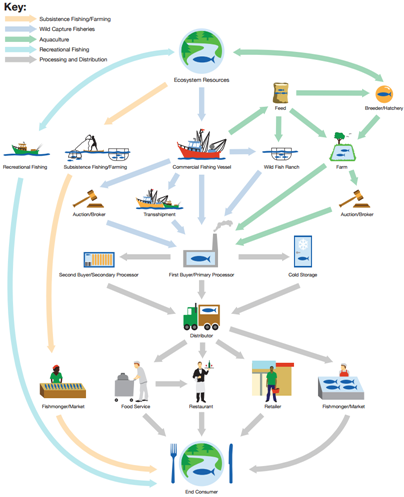
\includegraphics[scale=1.0]{figures/FishSupplyChain.png} \
   \caption{Source: \url{https://www.fishwise.org/images/fishwise_traceability_white_paper_august_2012.pdf}}
  \label{fig:supplychain}
\end{figure}

The supply chain through which fish are delivered is extremely complex (see Figure~\ref{fig:supplychain})
and involves diverse industries and regulatory controls that cross national boundaries. The
diversity of participants in the supply chain and the complex relationships between them makes this
a perfect opportunity of the use of blockchain technologies. A team at Intel is using the
Hyperledger Sawtooth blockchain technology to build a traceability prototype that combines the
distributed ledger, IoT sensors, and advanced communication technology to track telemetry parameters
such as location, temperature and humidity throughout capture, processing, and transit. Sensors
attached to the fish when it is caught record ownership and information about the location of the
catch in the ledger. Transactions on the ledger reflect interesting events in the processing of the
fish: ownership changes, transportation company, storage temperature range, etc. Further, analytics
on the ledger can be used for both regulatory enforcement and for scientific analysis of fish
harvesting and consumption.

The prototype highlights the benefits of Hyperledger Sawtooth as a platform for asset
traceability. The lightweight, highly decentralized consensus protocol in Sawtooth (``proof of
elapsed time'') is particularly well suited to the diverse, physically and organizationally
distributed ecosystem where potentially thousands of validating nodes are required. Broad
participation in the ledger reflects the cross-industry nature of the supply chain. Additionally,
asset tracking brings in a number of issues not generally seen in ledgers that focus on financial
products. For example, asset tracking requires handling of diverse data types such as the composite
format required for telemetry and environmental sensing. Transaction families in Sawtooth
accommodate domain-specific data and the transactions that operate on it, including enforcement of
data specific constraints (such as verification of the calibration of a sensor)

The use of blockchain technologies provides a number of benefits for cross-industry
traceability. Most importantly, blockchain technologies provide a means of establishing a public (to
the community of participants) and authoritative record of provenance. Its decentralized nature and
resiliency to faults enable updates from fishing boats, trucks, cold storage facilities and
restaurants. Beyond traceability, the digitization of assets (fish in this case) opens the doors for
completely new markets that might include, for example, monetization of provenance.


\subsection{Financial Services: Post Trade Activities}
The primary drivers for adoption of blockchain in financial service industry are considerations for privacy, confidentiality, and accountability. Compliance guidelines like “Anti Money Laundering” and “Know Your Customer” demand that users/customers are known and have been given clearance by their bank and/or the market infrastructure provider. These requirements drive the adoption of primarily permissioned and private blockchains as public blockchains still carry the risk of compromising participants' confidentiality and privacy. These considerations together with large volumes of transactions are the primary reasons that consortium blockchains are gaining momentum in adoption of distributed ledger technology by the financial services industry.

Among various use cases in financial services, and especially in capital markets, post trade activities is one of the prime areas, which can benefit from adoption of blockchain.

Post trade processing comprises all activities after the completion of a trade transaction. This general description is valid for all types of trading - OTC (over-the-counter)\footnote{OTC trading takes place when the trade counterparties interact directly or via brokerage services.} trading as well as trades executed at exchanges.

On a high level post-trade-processing comprises of the following operational steps:
\begin{description}
\item [Trade validation] - activities taking place following the trade execution, mainly validation and confirmation of the actual transactions amongst the trade participants or through exchange. 
\item [Clearing] - alignment and  matching of the actual trade instructions and confirmations across the different counterparties as well as potential netting activities. In case the counterparties have agreed on bilateral margining or the transactions are cleared through a clearing house, the counterparty/settlement risk arising between the time of concluding the trade and the time of settlement (typically 2 - 3 days) is mitigated. 
\item [Settlement] - the (legal) realization of the actual contractual obligations to reach the finality of the transaction. This includes support processes like the notification of all relevant entities affected by the transaction.
\item [Custody activities] - custodians are responsible for the safekeeping of securities. As such the positions held by the trade counterparties have to be adjusted. 
\end{description}

Besides these operational steps, post-trade-processing typically contains reporting requirements regarding the business transaction under consideration. Amongst these are counterparty internal risk reporting\footnote{The contribution of the transaction to the market and credit risk of the respective counterparts} and regulatory reporting. 

The operational steps as well as the reporting activities are in today’s setup typically a fragmented process chain spanning across a variety of departments of the respective counterparties, spread across a variety of entities, such as trade counterparties, brokers, settlement agents, central security depositories, clearing houses, thus resulting in a variety of interfaces. This consequently can result in a variety of reconciliation efforts along the process chain, between the trade counterparties as well as other entities/service providers involved, introducing inefficiencies in post trade processing.

Implementing post-trade-processing on blockchain is bound to lead to process efficiency gains as compared to the current implementation model. When settling via a blockchain system one could exploit the peer-to-peer property of a blockchain, i. e. one counterparty would insert the transaction details into the system and the other counterparty would verify and confirm.  Thus the confirmation processes would be processed within the same system, rendering separate confirmation processes obsolete.

In today’s world both parties would independently send their settlement instructions to a trusted 3rd party - the settlement agent - and this 3rd party would match both data sets and further process the settlement. Any mismatches in the initial instructions would lead to reconciliation efforts or even failed trades. In case of a blockchain solution, the network itself acts as an independent trusted 3rd party due to it's immutability and irrefutability of transactions.

The complexity of the multi-party interactions/interfaces is additionally reduced as all data from all from all process steps and actors resides on the blockchain and is accessible on a need-to-know basis. Therefore, the reconciliation processes should become obsolete altogether. Also the blockchain based system of record could serve as an efficient basis for reporting activities, e. g. regulatory transaction and trade reporting.

These efficiency gains have significant benefit to trade validation, clearing, both risk and regulatory reporting, as well as some aspects of the settlement phases of post trade processing\footnote{Using blockchain for near-time settlement may eliminate the netting (position offsetting) benefits to the counterparties derived from end-of-day processing, so its utility for the settlement portion of the post trade processing may be limited.}.

When looking to apply blockchain to financial services, in addition to the commonly recognized properties of a tamper-proof irrefutable transaction log, a blockchain used for post trace activity would need to have several features, typically achievable with the use of permissioned distributed ledgers.

Distributed ledgers used for capital markets use cases would typically be expected to have immediate finality. Nakamoto-style consensus algorithms (such as proof of work, proof of stake, or proof of elapsed time) may result in temporary forks, leading to transaction rollback, which is not acceptable for post trade processing use case. It is therefore expected that the blockchain applied here will have the ability to use a consensus algorithm, which has immediate finality.

Post trade activity participants have the expectation of privacy and confidentiality of transactions. The clearing house recording the transaction must ensure that parties are not able to perceive each others position and trade information. Moreover, the existence of trades themselves, even if parties are anonymized, should not be revealed since it may make transactions susceptible to traffic analysis. Current generation of analysis tools may be able to compromise both identity of the participants and trading patterns, which could be correlated to the public market information.

As described above current post trade activities happen at the end of the business day, thus presenting a different set of performance requirements than a system based on a blockchain would have. The total number of transactions would increase given the participants' ability to learn their position with the clearing house in near real-time. So while the average transactions per second number would increase, the peak performance requirements would decrease significantly, since end-of-day reconciliation used to transmit the entire set of trade records for the day would have been made obsolete.

\textbf{Hyperledger Fabric} channels combined with separate endorser sets provide an excellent solution to the problems of privacy and confidentiality. Ability to restrict data replication to only permissioned parties brings the benefits of the blockchain for data integrity and non-repudiation of transactions without compromising the security of the data. Additionally, reporting requirements - both internal and external - can be satisfied by including a regulatory agency and other oversight entities as members of the channel.

\textbf{Hyperledger Sawtooth} transaction families provide a reliable and performant way to encapsulate the operations relevant to the post trade. The ability to build complex rules using a language of choice to expose the interface which only provides the functions permitted in the context, bring a higher level of trust for the financial services institutions by providing the smart contract functionality without the risk of ad-hoc deployable code.

\textbf{Hyperledger Indy} provides an ability to have unlinkable verifiable claims, which can be leveraged to report outstanding risk on a shared ledger without compromising the identity of the firm, but still allow a regulatory body to have a holistic view of the market, enabling it to prevent potential market crashes and major defaults.


% section name in the file
\subsection{Health Records: Credentialing}

Blockchain technologies promise to reduce one of the great annoyances of
modern medical practice: ``credentialing''. Hospitals use the
credentialing process to make sure that its physicians are competent and
trustworthy. In a sense, credentialing is the hospital's way of
performing ``due diligence'' on a physician.

But today this process imposes a huge burden, both on the physician
applying for affiliation and the hospital that must vet the
applications.

\subsubsection{The physician gathers credentials, many on paper}

Any physician who wishes to become affiliated with a hospital begins the
process by gathering copies of all their professional credentials, such
as:

\begin{itemize}
\item Medical school diploma
\item Certificates of any residencies and fellowships completed
\item Certificates from any specialty medical boards
\item All state medical licenses
\item Evaluations from peers
\item Proof of meeting requirements for continuing medical education
\item Letters from hospitals where the physician was previously
      affiliated, explaining how and why  the affiliation ended
\item Details of any malpractice suits
\end{itemize}

\Mic{This paragraph is rather simplistic. Many of the required documents
are electronic, but simply not available. Some are paper hand must be
converted though often physical artifacts are used. My recommendation is
that we just get rid of this.}
Many of these documents were originally provided on paper, so the
physician may need to scan in paper copies, and manage a set of scanned
images or PDFs.

\subsubsection{The hospital checks credentials and calls a meeting}

On the hospital's side, the credentialing office checks the physician's
documentation for completeness, accuracy, and authenticity.  This is an
exacting task.  Almost inevitably, they find shortfalls and go back to
the doctor for missing documents.

Then the credentialing office verifies some or all of the physician's
documentation.  For example, they may phone a medical school to confirm
that the physician did indeed graduate from there.  This is clearly a
time-intensive process that is prone to errors.

Once the documentation is determined to be complete, accurate, and
authentic, the hospital's credentialing committee---which typically
includes physicians and administrators---meets to decide whether the
physician can begin practicing in affiliation with the hospital.

\Mic{Again, I'm not sure if calling out paper bound is either helpful or
accurate. I would prefer to simply leave it as ``complex''.}
The entire credentialing process is paper-bound, time-consuming, and
low-trust. And it can take weeks or even months until any physician is
cleared to affiliate with a hospital.

\subsubsection{Three key questions for any blockchain solution}

An effective blockchain solution for medical credentialing must answer
three key questions about content, identities, and resources.

\begin{enumerate}
\item Will actual content or only pointers to content be placed on the
blockchain?  Credentialing solutions might place public information
(such as state medical licensing) on the blockchain itself.  However,
private information (such as peer reviews) might be better stored off
the chain; this would guard against any loss of keys, and enable users
to remove---but not change---private information.

\item What's the best way to manage the identities of many participants?
An ambitious credentialing solution might include every hospital, every
physician, every source of continuing medical education, and so on.
This could eventually number thousands of participants.  How will so
many identities be efficiently and securely managed?

\item What resources are required, especially for storage?
Credentialing solutions may be in service for decades, requiring
significant resources for processing, communication, and storage.  For
example, what if at some point credentialing organizations want video
testimony from peers? Storage requirements could skyrocket---and who
would cover that added cost?
\end{enumerate}

\subsubsection{Hyperledger can help streamline credentialing}

Credentialing provides a good use case for blockchain technologies,
which can simplify and streamline every step of the process.

\textbf{Hyperledger Indy} provides off-the-shelf solutions that would
otherwise require architecting and developing new software. One
significant feature: Indy implements the proposed W3C standard for
verifiable claims, supporting the pairwise exchange of selected
credentials. In practice, this can work as follows:

\begin{enumerate}
\item A physician requests proof of graduation from their medical school.

\item The medical school places a digital credential on the blockchain
on behalf of the physician, where it's considered irrefutable and
tamper-proof.

\item A hospital can access the blockchain to verify the physician's
credential, with no need to contact the medical school directly.

\item The physician can expose only the specific credentials the
hospital requires, and nothing more.
\end{enumerate}

This implementation of verifiable claims safeguards the physician's
privacy, saves time and effort for everyone involved, and streamlines
the entire process. At last: a better way to handle medical
credentialing.



\section{Current Projects}
\subsection{Fabric}
Hyperledger Fabric (\url{https://github.com/hyperledger/fabric} and further repositories named like \url{fabric-*}) is a platform for distributed ledger solutions, underpinned by a modular architecture delivering high degrees of confidentiality, resiliency, flexibility and scalability. It is designed to support pluggable implementations of different components, and to accommodate the complexity and intricacies that exist across the economic ecosystem.

Starting from the premise that there are no ``one-size-fits-all'' solutions, Fabric is an extensible blockchain platform for running distributed applications.  It supports modular consensus protocols, which allows the system to be tailored to particular use cases and trust models. Fabric runs distributed applications written in general-purpose programming languages, without systemic dependency on a native cryptocurrency.  This stands in sharp contrast to most other blockchain platforms for running smart contracts that require code to be written in domain-specific languages or rely on a cryptocurrency.  Furthermore, it uses a portable notion of membership for realizing the permissioned model, which may be integrated with industry-standard identity management.  To support such flexibility, Fabric takes a novel architectural approach and revamps the way blockchains cope with non-determinism, resource exhaustion, and performance attacks.

%Where Hyperledger Fabric breaks from some other blockchain systems is that it is private and permissioned. Rather than allowing anyone to be part of the network by either participating in the Proof-of-Work consensus or receiving transferrable forms of data such as tokens over the blockchain, the members of a Hyperledger Fabric network enroll through a membership services provider.

Fabric also offers the ability to create channels, allowing a group of participants to create a separate ledger of transactions. This is an especially important option for networks where some participants might be competitors and not want every transaction they make, such as a special price they’re offering to some participants and not others, known to every participant in the network. If a group of participants form a channel, then only those participants, and no others, have copies of the ledger for that channel.



\subsection{Sawtooth}
Hyperledger Sawtooth (\url{https://github.com/hyperledger/sawtooth-core} and further repositories named like \url{sawtooth-*}) is a modular platform for building, deploying, and running distributed ledgers. The Sawtooth design philosophy targets keeping distributed ledgers distributed and making smart contracts safe - particularly for enterprise use.

In fitting with this enterprise focus, Sawtooth is also highly modular. This enables enterprises and consortia to make policy decisions that they are best equipped to make.

Originally, Sawtooth was designed to explore scalability, security, and privacy questions prompted by the original distributed ledgers. That mandated a certain modularity that was lacking at the time. Starting from scratch allowed us to employ lessons from those pioneering systems and branch into usages that the original currency ledgers weren’t intended to address. PoET, the new consensus hits scalability, while Transaction Families, our contract logic, narrow the attack surface for contracts while simultaneously broadening the functionality. We also have a keen interest in trusted execution environments and what role that can play in private transactions.

In branching into new business cases, we felt it was important that the system preserve certain tenants of a distributed ledger. That is, in an enterprise deployment, the concept of a distributed ledger shouldn’t collapse into a replicated database. Enterprise participants need autonomy and they have the right to run their own nodes. The set of participants will also be dynamic and the system – particularly consensus – must accommodate that volatility. It is not clear, for example, whether an O(n2) protocol with fixed membership like PBFT can support the scale or volatility of a distributed ledger at production levels. Further it seems inadvisable to sidestep the challenges of providing Byzantine Fault Tolerance and operate on only a Crash Fault Tolerant consensus. Finally, we observed that, “public” and “private” define a spectrum of authorization policies – not a binary option for a distributed ledger.


\subsection{Iroha}
Hyperledger Iroha (\url{https://github.com/hyperledger/iroha}) joined Hyperledger Fabric and Hyperledger Sawtooth to become the third distributed ledger platform under the Hyperledger umbrella in October, 2016. It was originally developed by Soramitsu in Japan and was proposed to Hyperledger by Soramitsu, Hitachi, NTT Data, and Colu.

Hyperledger Iroha is designed to be simple and easy to incorporate into infrastructural projects requires distributed ledger technology. Hyperledger Iroha features a simple construction; modern, domain-driven C++ design, emphasis on mobile application development and a new, chain-based Byzantine Fault Tolerant consensus algorithm, called Sumeragi. 

Iroha takes a very different design philosophy from Hyperledger Fabric and Hyperledger Sawtooth, in that it focuses on providing features that are helpful for creating applications for end-users. 


\subsection{Burrow}
Hyperledger Burrow is a permissionable smart contract machine; it became the fourth distributed ledger platform under the Hyperledger umbrella in April, 2017. It was originally developed and proposed to Hyperledger by Monax. 

Burrow provides a modular blockchain client with a permissioned smart contract interpreter built to the specification of the Ethereum Virtual Machine (EVM). Burrow provides a strongly deterministic, smart contract focused, blockchain design to Hyperledger's overall effort. Users of Burrow are able to benefit from having an access control layer through the use of smart contracts and our “secure natives” based permission layer. 
 
The major components of Burrow are as follows:
 
Consensus engine which is responsible for maintaining the networking stack between nodes and ordering transactions to be utilized by the application engine.
Application Blockchain Interface (“ABCI”) provides the interface specification for the consensus engine and application engine to connect.
Smart contract application engine provides application builders with a strongly deterministic smart contract engine for operating complex industrial processes.
Gateway provides programmatic interfaces for systems integrations and user interfaces


\subsection{Indy}
Hyperledger Indy uses distributed ledger technology to make identity independent of organizational silos; friends, competitors, and even antagonists can all rely on a shared source of truth that answers fundamental questions such as, “Who am I dealing with?” and “How can I verify data about the other party in this interaction?” Solid answers to these questions enable the sort of trusted interactions demanded everywhere.

Because Indy stores identity artifacts (public keys, proofs of existence, cryptographic accumulators that enable revocation) on a ledger with distributed ownership, identities can be self-sovereign--nobody external to the identity owner can manipulate them or take them away. Identity in Indy is also privacy-preserving by default, meaning that an identity owner can operate without creating correlation risk or breadcrumbs.

A core technology for Indy is verifiable claims. These attestations of an identity’s attributes resemble credentials familiar to all of us: passports, driver’s licenses, birth certificates, and so forth. But they can be combined and transformed in powerful ways, using zero-knowledge proofs to enable selective disclosure of just those pieces of data that a particular context demands.

This combination of self-sovereignty, privacy, and verifiable claims is synergistic. Bulk troves of sensitive data vanish or become useless. The economics of hacking transform. The competing demands of privacy-preserving and strongly identifying regulations are satisfied. Individuals and organizations are free to seek mutual benefit from rich interaction; the identity ecosystem gains the innovation and dynamism of a free market. 

Despite the advanced crypto under the hood, Indy’s API is simple and straightforward. It consists of about 50 C-callable functions, with idomatic wrappers for many mainstream programming languages, 



\subsection{Cello}
Hyperledger Cello is an open framework to help people adopt blockchain technologies efficiently and easily, by providing automatic ways in blockchain provision and operational management. 

It brings the on-demand "as-a-service" deployment model to the blockchain ecosystem to reduce the effort required for maintaining the lifecycle of the Hyperledger blockchain frameworks. It provides a multi-tenant chain service efficiently and automatically on top of various infrastructures, including baremetal, virtual machine, Cloud platforms like AWS, and container platforms like Docker Swarm and Kubernetes, overall helping provide "Blockchain as a Service" efficiently. It also helps with maintainance through a dashboard where users can watch the statistics/status of the blockchain system (e.g., system utilization, blockchain events, chaincode performance), and manage the blockchains (e.g., create, config and delete) and chaincode (e.g., deploy and upload private chaincode) in real-time.

Hyperledger Cello currently supports Hyperledger Fabric 1.0 as the main blockchain implementation, while it has plans to support more blockchain types like sawtooth. The architecture follows the micro-service style, with pluggable implementations for most components. The main programing languages are Python and JavaScript.


\subsection{Composer}
TODO.

\subsection{Explorer}
Hyperledger Explorer (\url{https://github.com/hyperledger/blockchain-explorer}) provides a dashboard for viewing information about transactions, blocks, node logs, statistics,  and smart contracts available on the network. Users will be able to query for specific blocks or transactions and view the complete details. Blockchain explorer can also be integrated with any authentication/authorization platforms (commercial/open source) and will provided appropriate functionality based on the privileges available to the user. 
Goals of the project are listed below.
To implement a generic Blockchain explorer web application which is easy to install and can be used with different Blockchain platforms.
Use latest tools and technologies that make the explorer easy to implement, maintain and extend.
Easily installable package available through standard package managers for most popular platforms.

%Please refer to the project proposal document on the wiki (\url{https://wiki.hyperledger.org/projects/explorer}) page to understand more about the project.


\section{Highlighted Features}
\subsection{Identity}
Indy shares some features with traditional enterprise identity solutions--the world of LDAP, OAuth, 2FA, IDPs, and similar tech. Both approaches use industrial-strength crypto. Both enable capturing and sharing rich metadata about an identity. Both facilitate sophisticated access control and policy. But there is a profound difference: Indy identities are shared instead of siloed and federated. An Indy identity is portable--you can bring it with you wherever the distributed ledger is accepted. Ten orgs or systems that each support Indy identities don't create ten separate identities for John Q. Public; John simply shows up with his pre-existing identity and uses it. Organizations can cancel John's access, but never his identity, because John owns it. John, not the places that accept John's identity, controls access to his data.

Indy also shares some features with blockchain-based identity solutions such as Blockstack and Uport. All of these technologies store identity on a distributed ledger and thus promote security and personal freedom. However, Blockstack and Uport depend on Bitcoin and Ethereum, respectively. These are proof-of-work ecosystems that impose a non-trivial cost on transactions; every new persona, public key rotation, published attribute, or pairwise relationship is a tangible expense. This creates a disincentive to pairwise relationships, which undermines privacy. Also, these ecosystems are global and public; they cannot be special-purposed for a less-than-fully-global context. Indy, on the other hand, does not use proof-of-work. Transactions are free. And different instances of Indy can be used in whatever context is convenient.


\section{Long-Term Vision}
We already live in a highly interconnected world. In the future, we believe that the world will become even more closely tied together: more data sharing, more communication, and more digital content will become the norm in both business and personal lives. This will necessitate careful management of security, privacy, and trust. We view distributed ledger technology as the solution to the problem where someone needs a distributed database for which there is no single owner that is trusted by all of the users. Thus, as interconnection increases, we believe that blockchain and DLT will become quite prevalent in society as distributed ledgers replace some (but not all) traditional databases.

This prevalence of distributed ledgers will not come about without difficulty, however. Nothing in this space is `for free'--for instance, if you want a great deal of security and privacy features in a blockchain, you will often pay the price in terms of performance. This implies that we will need to have a large variety of different blockchains--no one blockchain will work for all applications--that can communicate and interact seamlessly.

Thus, our long-term vision for Hyperledger is driven by two main architectural concerns: modularity and interoperability. We hope that, eventually, Hyperledger consists of lots of modules for various different blockchain components that can be put together by a non-expert into a cohesive, functional, and secure distributed ledger. All of these modules would be interchangeable with other modules of the same time, and able to communicate with other modules of different types (or the same type if involved in communication between separate blockchains). This would ideally enable a non-expert to set up an interoperable, secure blockchain quickly, easily, and efficiently.

We want to specifically point out that we do not believe Hyperledger should be the `one distributed ledger to rule them all'. The technical community of Hyperledger sees merit in many diverse blockchains, and, while we hope that other developers consider interoperability with Hyperledger.  We do not intend for Hyperledger to be a single stack. Instead, we hope that it becomes a collection of tools purpose built with interoperability and modularity in mind. Any individual can use one, some, or all of the Hyperledger projects to to create a distributed ledger to suit their needs.

In the future, we hope that Hyperledger can solve most of the common problems in the distributed ledger space. This will necessitate a good community, strong industrial support, and solid design principles, and, as we have hopefully illustrated in this paper, we have structured Hyperledger with these tenets in mind. It is now up to us to go out and accomplish this.


\section{Conclusion}
TODO.

\iftoggle{fullversion}{
    \bibliographystyle{alpha}
}{
    \bibliographystyle{alpha}
}
\bibliography{hyperledger}

\clearpage
%\appendix
\iftoggle{fullversion}{}{
%\input{appendix.tex}
}
%\input{appendixtwo.tex}
\iftoggle{fullversion}{}{
%\input{appendixthree.tex}
}

\end{document}
